
\section{Bias Variance}

\begin{frame}
    \frametitle{Expected Generalization Error}
    Let $D = \{(x_{1},y_{1}), (x_{2}, y_{2}), ... , (x_{N}, y_{N})\}$ and  $y = f(x) + \epsilon$. \\
       
    The decomposition of a model's expected generalization error is
    \begin{equation}
        \boldsymbol{Err}(f(x)) = Noise(x) + [Bias(\hat{f}(x))]^2 + Var(\hat{f}(x))
    \end{equation}
    
    $Noise$ is irreducible and independent of the model. \\
    There is a trade-off between $bias^2$ and variance. \\
    Adjusting parameters to decrease variance increases $bias^2$ and vice versa.
\end{frame}

\begin{frame}
    \frametitle{Bias-Variance Trade-off}
    \begin{figure}      
        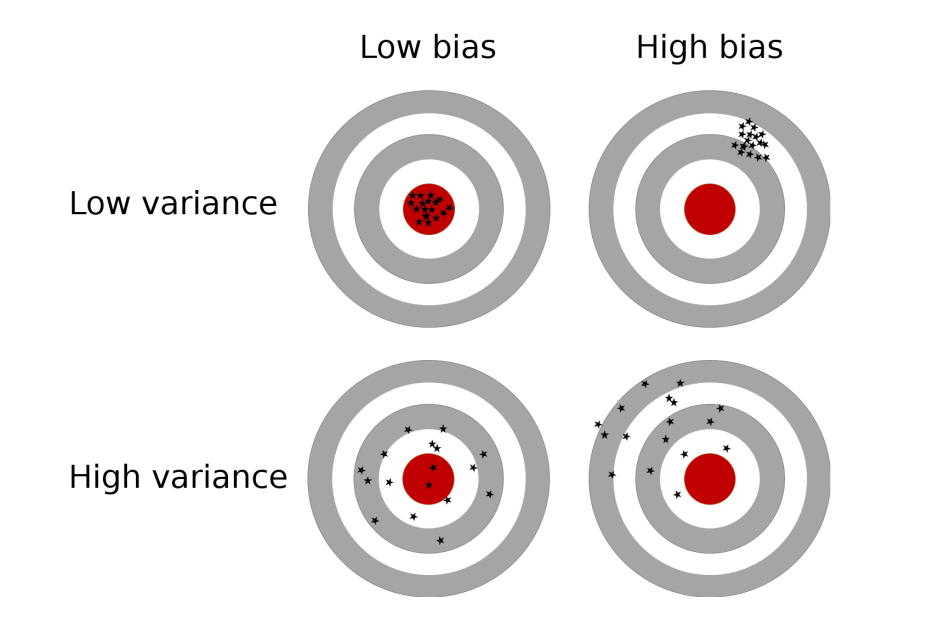
\includegraphics{images/bias-variance.png}
        \caption{Illustration of bias-variance trade-off \cite{van2019bias}}
    \end{figure}
    Decision trees generally have low bias and high variance \cite{friedman2001elements}.

\end{frame}

    %\begin{columns}[c] % The "c" option specifies centered vertical alignment while the "t" option is used for top vertical alignment
    
    %\column{.45\textwidth} % Left column and width
    %\textbf{Heading}
    %\begin{enumerate}
    %\item Statement
    %\item Explanation
    %\item Example
    %\end{enumerate}
    
    %\column{.5\textwidth} % Right column and width
    %Lorem ipsum dolor sit amet, consectetur adipiscing elit. Integer lectus nisl, ultricies in feugiat rutrum, porttitor sit amet augue. Aliquam ut tortor mauris. Sed volutpat ante purus, quis accumsan dolor.
    
    %\end{columns}
